\begin{lstlisting}
•    Section 8.1:  1,  4,  6,  9, 10  
•    Section 8.2:  2,  7,  11,  12(a)(b)(C),  13
\end{lstlisting}
\begin{exercise}
\begin{figure}[H]
\centering
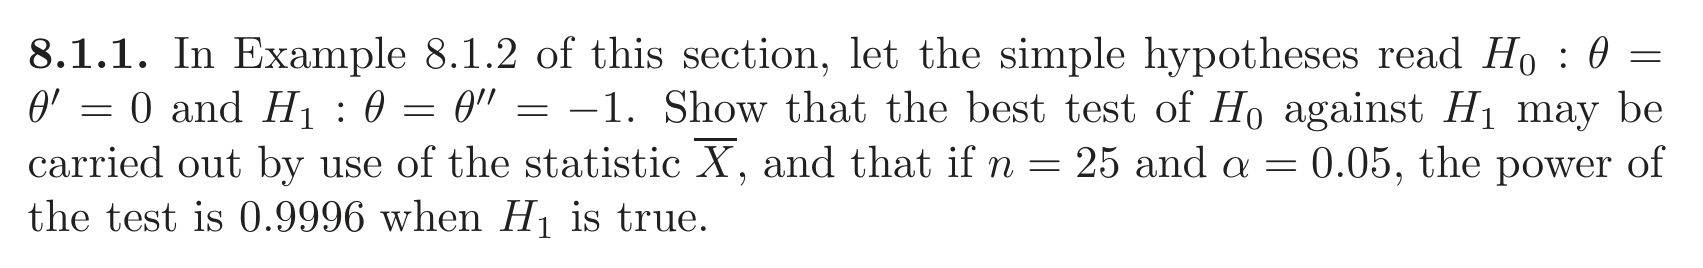
\includegraphics[width=\textwidth]{9-hw14-2025060521.png}
% \caption{}
\label{}
\end{figure}
\end{exercise}
\[
\begin{aligned}
\frac{L\left(\theta^{\prime} ; \mathbf{x}\right)}{L\left(\theta^{\prime \prime} ; \mathbf{x}\right)} & =\frac{(1 / \sqrt{2 \pi})^n \exp \left[-\sum_1^n x_i^2 / 2\right]}{(1 / \sqrt{2 \pi})^n \exp \left[-\sum_1^n\left(x_i+1\right)^2 / 2\right]} \\
& =\exp \left(\sum_1^n x_i+\frac{n}{2}\right)
\end{aligned}
\]
By Neyman-Pearson Theorem, the best test of $H_0$ against $H_1$ can be given by ($k>0$)
\[
\frac{L\left(\theta^{\prime} ; \mathbf{x}\right)}{L\left(\theta^{\prime \prime} ; \mathbf{x}\right)} \leq k \text { for each } \mathbf{x} \in C
\]
i.e.
\[
\exp\left( n\overline{X}+\frac{n}{2} \right)\leq k
\]
i.e.
\[
\overline{X}\leq \frac{1}{n}\log k-\frac{1}{2}\eqqcolon c
\]
In this case, a best critical region is the set $C=\{ (x_1,\dots,x_n):\overline{X}\leq c \}$.
\[
\alpha=\mathbb{P}_{H_0}(\overline{X}\leq c)
\]
Let $n=25$, $\alpha=0.05$, then under $H_0$, $X_i\sim N(0,1)$, $\overline{X}\sim N\left( 0,\frac{1}{25} \right)$, then $0.05=\mathbb{P}_{H_0}(5\overline{X}\leq5c)$, $c=\frac{1}{5}\Phi ^{-1}(0.05)=-0.328971$. Then the probability of rejecting $H_0$, when $H_0$ is false, is the power of the test at $H_1$, which is
\[
\mathbb{P}_{H_1}(\overline{X}\leq c)=\int_{-\infty}^{c} \frac{1}{\sqrt{ 2\pi }\cdot\frac{1}{5}}\exp\left[ -\frac{(x+1)^2}{\frac{2}{25} } \right] \, \mathrm{d}x =0.999603
\]
\begin{lstlisting}[language=mathematica]
(*定义一个概率 p*)p = 0.05;

(*使用 Quantile 求标准正态分布的逆函数*)
c = Quantile[NormalDistribution[0, 1], p]/5

Integrate[(1/(Sqrt[2 Pi]*(1/5)))* Exp[-((x + 1)^2/(2/25))], {x, -Infinity, c}]
\end{lstlisting}
\begin{exercise}
\begin{figure}[H]
\centering
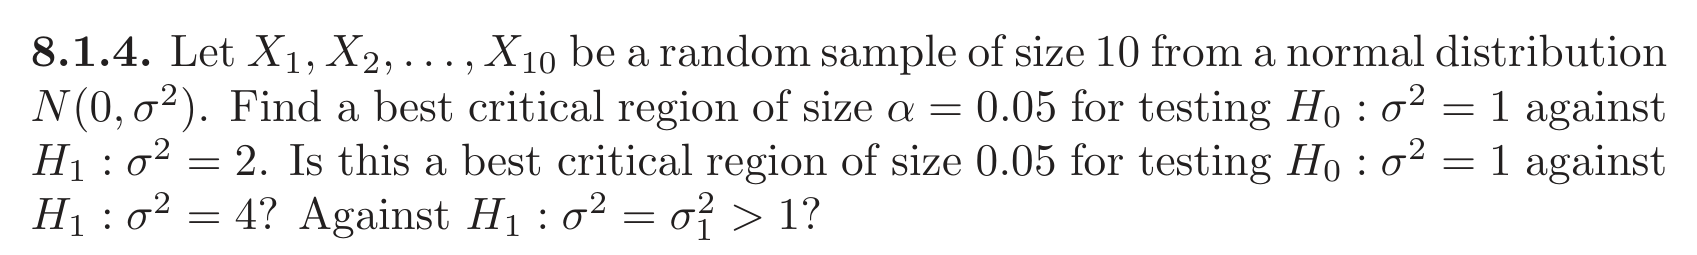
\includegraphics[width=\textwidth]{8-hw14-2025060521.png}
% \caption{}
\label{}
\end{figure}
\end{exercise}
For $H_1:\sigma^{2}=2$,
\[
\frac{L(\sigma^{2}=1;\mathbf{x})}{L(\sigma^{2}=2;\mathbf{x})}=\frac{(2\pi)^{-5}\cdot \exp\left( -\frac{1}{2}\sum_{i=1}^{10} x_i^2 \right)}{(2\pi)^{-5}\cdot2^{-5}\cdot \exp \left( -\frac{1}{4} \sum_{i=1}^{10} x_i^2\right)}=32\exp\left( -\frac{1}{4}\sum_{i=1}^{10} x_i^2 \right)
\]
By Neyman-Pearson Theorem, the best test of $H_0$ against $H_1$ can be given by ($k>0$)
\[
32\exp\left( -\frac{1}{4}\sum_{i=1}^{10} x_i^2 \right)\leq k
\]
i.e.
\[
\sum_{i=1}^{10} X_i^2\geq  -4\log(k/32)\eqqcolon c
\]
In this case, a best critical region is the set $C=\left\{  (x_1,\dots,x_n):\sum X_i^2\geq c  \right\}$.
\[
\alpha=\mathbb{P}_{H_0}\left( \sum_{i=1}^{10} X_i^2\geq c \right)
\]
where $\sum_{i=1}^{10}X_i^2\sim \chi^{2}(10)$. Then $c=\Phi ^{-1}_{\chi^{2}(10)}(1-\alpha)=18.307$. The critical region is
\[
\left\{  \sum_{i=1}^{10} X_i^2\geq 18.307  \right\}
\]
\begin{lstlisting}[language=mathematica]
(* 定义自由度 *) nu = 10; (* 定义一个概率 p *) p = 0.95; (* 使用 Quantile 求卡方分布的逆函数 *) x = Quantile[ChiSquareDistribution[nu], p]
\end{lstlisting}
For $H_1:\sigma^{2}=4$, the critical region is also
\[
\left\{  \sum_{i=1}^{10} X_i^2\geq 18.307  \right\}
\]
For $H_1:\sigma^{2}=\sigma_1^2>1$,
\[
\frac{L(\sigma^{2}=1;\mathbf{x})}{L(\sigma^{2}=\sigma_1^2;\mathbf{x})}=\frac{(2\pi)^{-5}\cdot \exp\left( -\frac{1}{2}\sum_{i=1}^{10} x_i^2 \right)}{(2\pi)^{-5}\cdot\sigma_1^{-5}\cdot \exp \left( -\frac{1}{2\sigma_1^2} \sum_{i=1}^{10} x_i^2\right)}=\sigma_1^{5}\exp\left( -\frac{1}{2}\left(1- \frac{1}{\sigma_1^2} \right)\sum_{i=1}^{10} x_i^2 \right)
\]
By Neyman-Pearson Theorem, the best test of $H_0$ against $H_1$ can be given by ($k>0$)
\[
\sigma_1^{5}\exp\left( -\frac{1}{2}\left(1- \frac{1}{\sigma_1^2} \right)\sum_{i=1}^{10} x_i^2 \right)\leq k
\]
i.e.
\[
\sum_{i=1}^{10} X_i^2\geq -\frac{2\sigma_1^2}{\sigma_1^2-1}\log \left( \frac{k}{\sigma_1^{5}} \right) \eqqcolon c
\]
The critical region is also
\[
\left\{  \sum_{i=1}^{10} X_i^2\geq 18.307  \right\}
\]
\begin{exercise}
\begin{figure}[H]
\centering
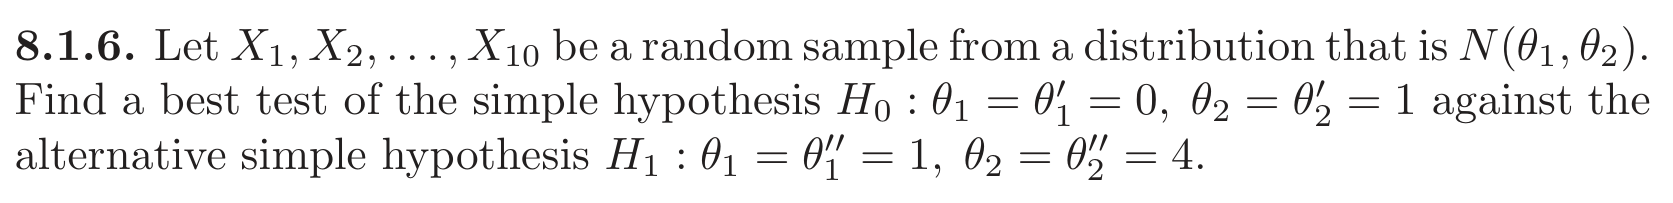
\includegraphics[width=\textwidth]{7-hw14-2025060521.png}
% \caption{}
\label{}
\end{figure}
\end{exercise}
\[
\begin{aligned}
\frac{L(\boldsymbol{\theta}';\mathbf{x})}{L(\boldsymbol{\theta}'';\mathbf{x})} & =\frac{\prod_{i=1}^{10}(2\pi\theta_2')^{-1/2 }\exp \{ -(x_i-\theta_1')^2/(2\theta_2') \} }{\prod_{i=1}^{10}(2\pi\theta_2'')^{-1/2 }\exp \{ -(x_i-\theta_1'')^2/(2\theta_2'')} \\
 & =\frac{(2\pi)^{-5}\exp \left\{  -\frac{1}{2}\sum_{i=1}^{10} x_i^2  \right\}}{(4\pi)^{-5}\exp \left\{  -\frac{1}{8}\sum_{i=1}^{10} (x_i-1)^2  \right\}} \\
 & =32\exp \left\{ -\frac{3}{8}\sum_{i=1}^{10} X_i^{2}-\frac{1}{4}\sum_{i=1}^{10} X_i+\frac{5}{4} \right\} 
\end{aligned}
\]
By Neyman-Pearson Theorem, the best test of $H_0$ against $H_1$ can be given by ($k>0$)
\[
32\exp \left\{ -\frac{3}{8}\sum_{i=1}^{10} X_i^{2}-\frac{1}{4}\sum_{i=1}^{10} X_i+\frac{5}{4} \right\} \leq k
\]
i.e.
\[
\frac{3}{8}\sum_{i=1}^{10} X_i^{2}+\frac{1}{4}\sum_{i=1}^{10} X_i\geq \frac{5}{4}-\log\left( \frac{k}{32} \right)\eqqcolon c
\]
\begin{exercise}
\begin{figure}[H]
\centering
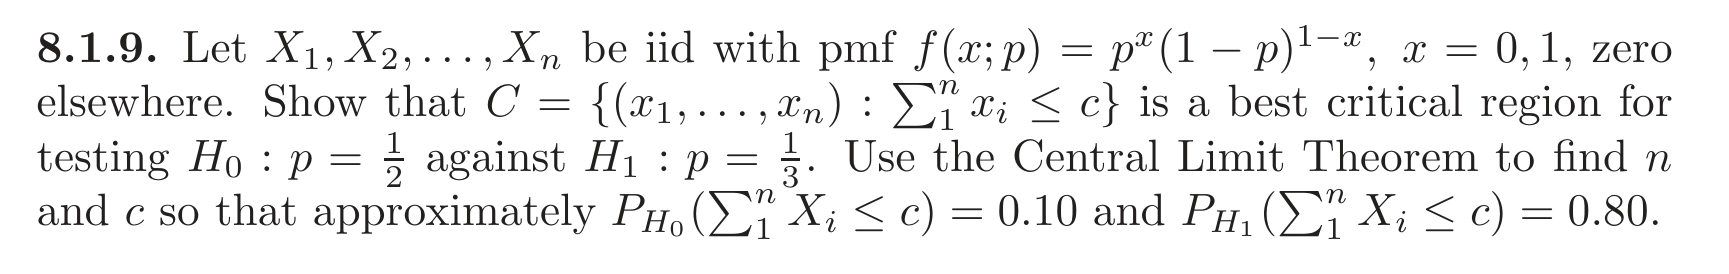
\includegraphics[width=\textwidth]{6-hw14-2025060521.png}
% \caption{}
\label{}
\end{figure}
\end{exercise}
$p'=\frac{1}{2},p''=\frac{1}{3}$, then
\[
\frac{L(p';\mathbf{x})}{L(p'';\mathbf{x})}=\frac{\prod_{i=1}^{n} p'^{x_i}(1-p')^{1-x_i}}{\prod_{i=1}^{n} p''^{x_i}(1-p'')^{1-x_i}}=\left( \frac{3}{4} \right)^{n}\cdot2^{\sum_{i=1}^{n} x_i}
\]
By Neyman-Pearson Theorem, the best test of $H_0$ against $H_1$ can be given by ($k>0$)
\[
\left( \frac{3}{4} \right)^{n}\cdot2^{\sum_{i=1}^{n} x_i}\leq k
\]
i.e.
\[
\sum_{i=1}^{n} X_i\leq \frac{1}{\log2}\left( \log k-n\log\frac{3}{4} \right)\eqqcolon c
\]
By CLT, $Y_n\coloneqq\left( \sum_{i=1}^{n}X_i-np \right)/(\sqrt{ n p(1-p)})$ has an approximate distribution $N(0,1)$. Then
\[
\mathbb{P}_{H_0}\left( \sum_{i=1}^{n} X_i\leq c \right)=\mathbb{P}_{H_0}\left( Y_n\leq \frac{c-np}{\sqrt{ np(1-p) }} \right)=\Phi\left( \frac{c-\frac{n}{2}}{\sqrt{ \frac{n}{4} }} \right)=\Phi \left( \frac{2c-n}{\sqrt{ n }} \right)
\]
\[
\mathbb{P}_{H_1}\left( \sum_{i=1}^{n} X_i\leq c \right)=\Phi\left( \frac{c-\frac{n}{3}}{\sqrt{ \frac{2n}{9} }} \right)=\Phi\left( \frac{3c-n}{\sqrt{ 2n }} \right)
\]
We have
\[
\begin{aligned}
c & =\frac{1}{2}[n+\sqrt{ n }\Phi ^{-1}(0.10)] \\
c & =\frac{1}{3}[n+\sqrt{ 2n }\Phi ^{-1}(0.80)]
\end{aligned}
\]
where $\Phi ^{-1}(0.10)=-1.28155, \Phi ^{-1}(0.80)=0.841621$. Solve the equation then we get
\[
c=15.3871,\quad n=38.7521
\]
\begin{lstlisting}[language=mathematica]
(*定义一个概率 p*)p = 0.10;

(*使用 Quantile 求标准正态分布的逆函数*)
x = Quantile[NormalDistribution[0, 1], p]
\end{lstlisting}
\begin{exercise}
\begin{figure}[H]
\centering
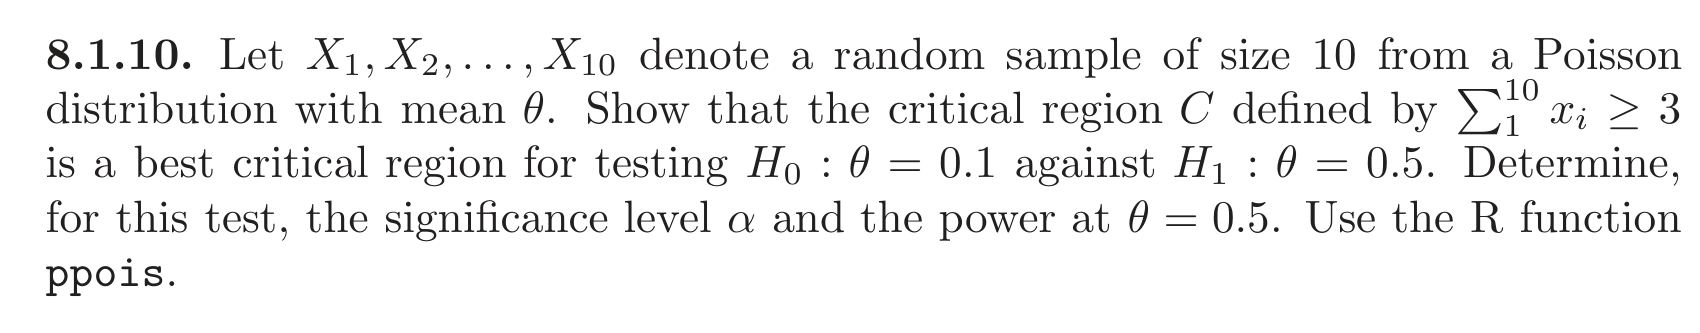
\includegraphics[width=\textwidth]{5-hw14-2025060521.png}
% \caption{}
\label{}
\end{figure}
\end{exercise}
$\theta'=0.1$, $\theta''=0.5$ then
\[
\frac{L(\theta';\mathbf{x})}{L(\theta'';\mathbf{x})}=\frac{\prod_{i=1}^{10} \frac{\theta'^{x_i}}{x_i!}e^{ -\theta' }}{\prod_{i=1}^{10} \frac{\theta''^{x_i}}{x_i!}e^{ -\theta'' }}=e^{ 10(\theta''-\theta') }\cdot\left( \frac{\theta'}{\theta''} \right)^{\sum_{i=1}^{10} x_i}=e^{ 4 }\cdot5^{-\sum_{i=1}^{10} x_i}
\]
By Neyman-Pearson Theorem, the best test of $H_0$ against $H_1$ can be given by ($k>0$)
\[
e^{ 4 }\cdot5^{-\sum_{i=1}^{10} x_i}\leq k
\]
i.e.
\[
\sum_{i=1}^{10} X_i\geq -\frac{1}{\log5}\log(ke^{ -4 })\eqqcolon c
\]
The critical region $C$ defined by $\sum_{i=1}^{10}x_i\geq3$ is of the form, thus is a best critical region. We have $\sum_{i=1}^{10}X_i\sim \mathrm{Poi}(10\theta)$, then under $H_0$, $\sum_{i=1}^{10}X_i\sim\text{Poi}(1)$.
\[
\alpha=\mathbb{P}_{H_0}\left( \sum_{i=1}^{10} X_i\geq 3 \right)=1-\frac{5}{2e}
\]
The power at $\theta=0.5$ is (under $H_1$, $\sum_{i=1}^{10}X_i\sim\text{Poi}(5)$)
\[
\mathbb{P}_{H_1}\left( \sum_{i=1}^{10} X_i\geq 3 \right)=1-\frac{37}{2e^{ 5 }}
\]
\begin{exercise}
\begin{figure}[H]
\centering
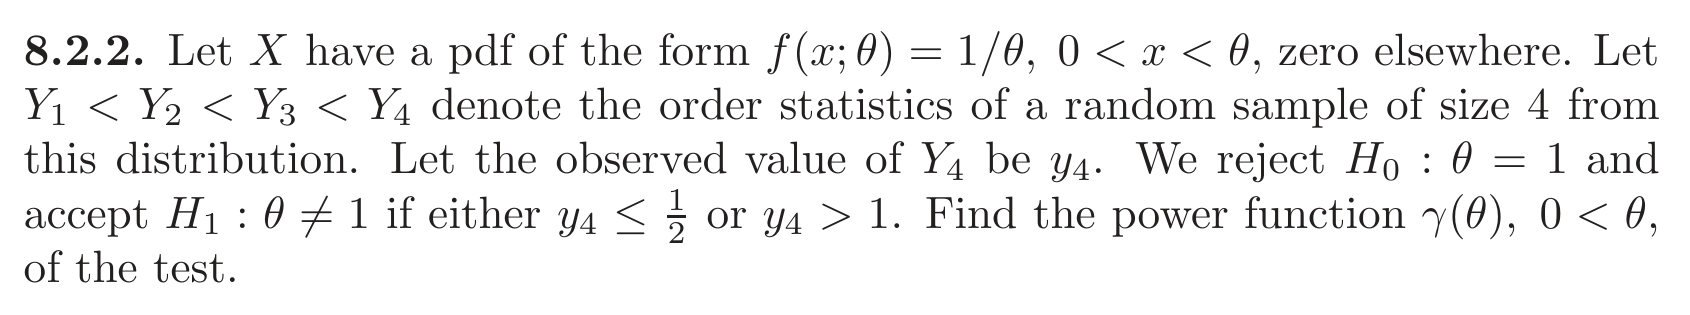
\includegraphics[width=\textwidth]{4-hw14-2025060521.png}
% \caption{}
\label{}
\end{figure}
\end{exercise}
\[
C\coloneqq \left\{  y_4\leq \frac{1}{2}\text{ or }y_4>1  \right\}
\]
\[
\gamma(\theta)=\mathbb{P}_{H_1}(\mathbf{Y}\in C)=\mathbb{P}_{H_1}\left( Y_4\leq\frac{1}{2}  \right)+\mathbb{P}_{H_1}(Y_4>1)=\begin{cases}
\frac{1}{16} \theta^{-4} & 0<\theta< 1 \\
1-\frac{15}{16} \theta^{-4} & \theta>1
\end{cases}
\]
\begin{exercise}
\begin{figure}[H]
\centering
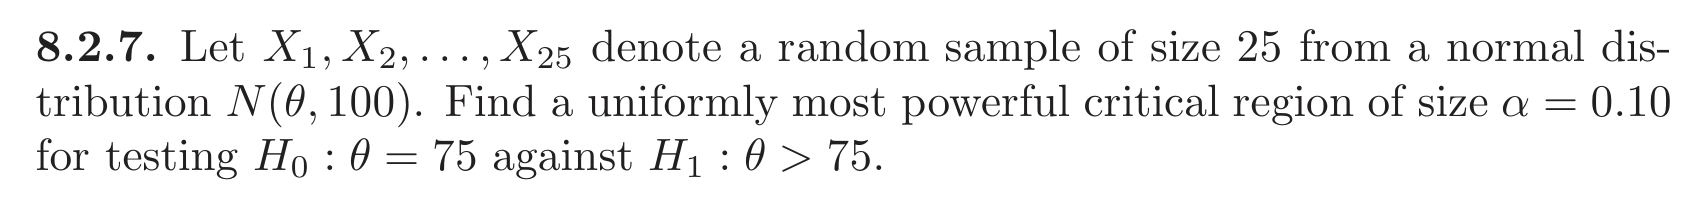
\includegraphics[width=\textwidth]{3-hw14-2025060521.png}
% \caption{}
\label{}
\end{figure}
\end{exercise}
\[
\begin{aligned}
L(\theta;\mathbf{x}) & =\prod_{i=1}^{25} (20\pi)^{-1/2 }\exp \{ -(x_i-\theta)^2/200 \}  \\
 & =(20\pi)^{-\frac{25}{2}}\exp \left\{  -\frac{1}{200}\sum_{i=1}^{25} x_i^{2}+\frac{\theta}{100} \sum_{i=1}^{25} x_i-\frac{1}{8}\theta^{2}   \right\}
\end{aligned}
\]
Let $\theta''$ represent a number greater than $\theta'=75$, and $k$ denote a positive number. Let $C$ be the set of points where
\[
\frac{L(\theta';\mathbf{x})}{L(\theta'';\mathbf{x})}=\exp \left\{  \frac{\theta'-\theta''}{100}\sum_{i=1}^{25} X_i-\frac{1}{8}(\theta'^{2}-\theta''^{2})  \right\}\leq k
\]
i.e.
\[
\overline{X}=\frac{1}{25} \sum_{i=1}^{25} X_i\geq   \frac{4}{\theta'-\theta''}\log k+\frac{1}{2}(\theta'+\theta'')\eqqcolon c
\]
The set $C=\left\{  (x_1,\dots,x_{25}):\frac{1}{25}\sum_{i=1}^{25}x_i\geq c  \right\}$ is then a best critical region for testing the simple hypothesis $H_0:\theta=\theta'$ against the simple hypothesis $\theta=\theta''$. It remains to determine $c$, so that this critical region has the desired size $\alpha$.

If $H_0$ is true, the r.v. $\overline{X}\sim N(75,4)$. Let
\[
\alpha=\mathbb{P}_{H_0}(\overline{X}\geq c)=\mathbb{P}_{H_0}\left( \frac{\overline{X}-75}{2}\geq \frac{c-75}{2} \right)=1-\Phi\left( \frac{c-75}{2} \right)
\]
then $c=75+2\cdot\Phi ^{-1}(1-\alpha)=1.28155$. Then $C=\left\{  (x_1,\dots,x_{25}):\overline{x}\geq1.28155  \right\}$ is a best critical region of size $\alpha$ for testing $H_0:\theta=\theta'$ against the hypothesis $\theta=\theta''$. Moreover, for each number $\theta''$ greater than $\theta'$, the foregoing argument holds. Thtat is, $C$ is a uniformly most powerfull critical region.

\begin{exercise}
\begin{figure}[H]
\centering
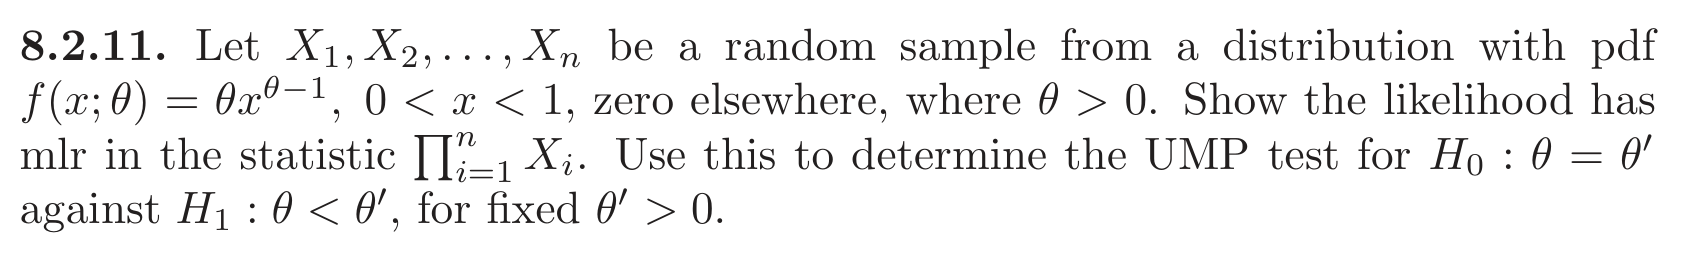
\includegraphics[width=\textwidth]{2-hw14-2025060521.png}
% \caption{}
\label{}
\end{figure}
\end{exercise}
\[
L(\theta;\mathbf{x}) = \prod_{i=1}^{n} \theta x_i^{\theta-1}=\theta^{n}\left( \prod_{i=1}^{n} x_i \right)^{\theta-1}
\]
Let $\theta''$ represent a number greater than $\theta'$, and $k$ denote a positive number. Let $C$ be the set of points where
\[
\frac{L(\theta';\mathbf{x})}{L(\theta'';\mathbf{x})}=\left( \frac{\theta'}{\theta''} \right)^{n}\left( \prod_{i=1}^{n} x_i \right)^{\theta'-\theta''}\leq k
\]
thus the likelihood has mlr in the statistic $\prod_{i=1}^{n}X_i$.

i.e.
\[
\prod_{i=1}^{n} x_i\leq \left( k\cdot\left( \frac{\theta''}{\theta'} \right)^{n} \right)^{1/(\theta'-\theta'')}\eqqcolon c
\]
UMP test: Reject $H_0$ if $\prod_{i=1}^{n}X_i\leq c$.

\begin{exercise}
\begin{figure}[H]
\centering
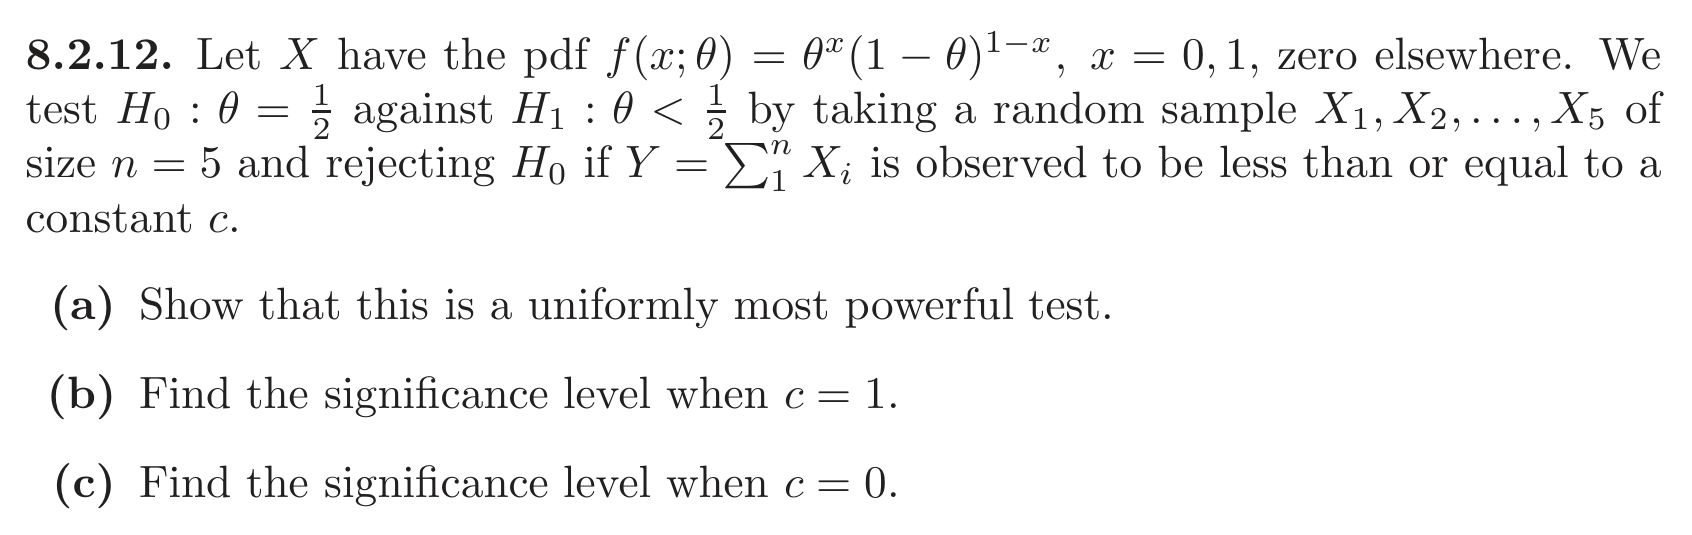
\includegraphics[width=\textwidth]{1-hw14-2025060521.png}
% \caption{}
\label{}
\end{figure}
\end{exercise}
(a)
\[
f(x;\theta)=\exp \left\{  x\log\frac{\theta}{1-\theta}-\log(1-\theta)  \right\}
\]
$\log\frac{\theta}{1-\theta}$ is increasing for $\theta\in\left( 0,\frac{1}{2}\right]$, then a UMPT is rejecting $H_0$ if $\sum_{i=1}^{n}X_i\leq c$.

(b)
$X_i\sim b (1,\theta)$, then $Y\sim b(n,\theta)$, $p(x)=\binom{n}{x}\theta^{x}(1-\theta)^{n-x}$.

When $n=5$, under $H_0$, $p(x)=\binom{5}{x}\cdot2^{-5}$, where $x=0,1,\dots,5$.

The significance level is
\[
\alpha=\mathbb{P}_{H_0}(Y\leq 1)=(1+5)\cdot2^{-5}=\frac{3}{16}
\]
(c)
\[
\alpha=\mathbb{P}_{H_0}(Y\leq 0)=\frac{1}{32} 
\]
\begin{exercise}
\begin{figure}[H]
\centering
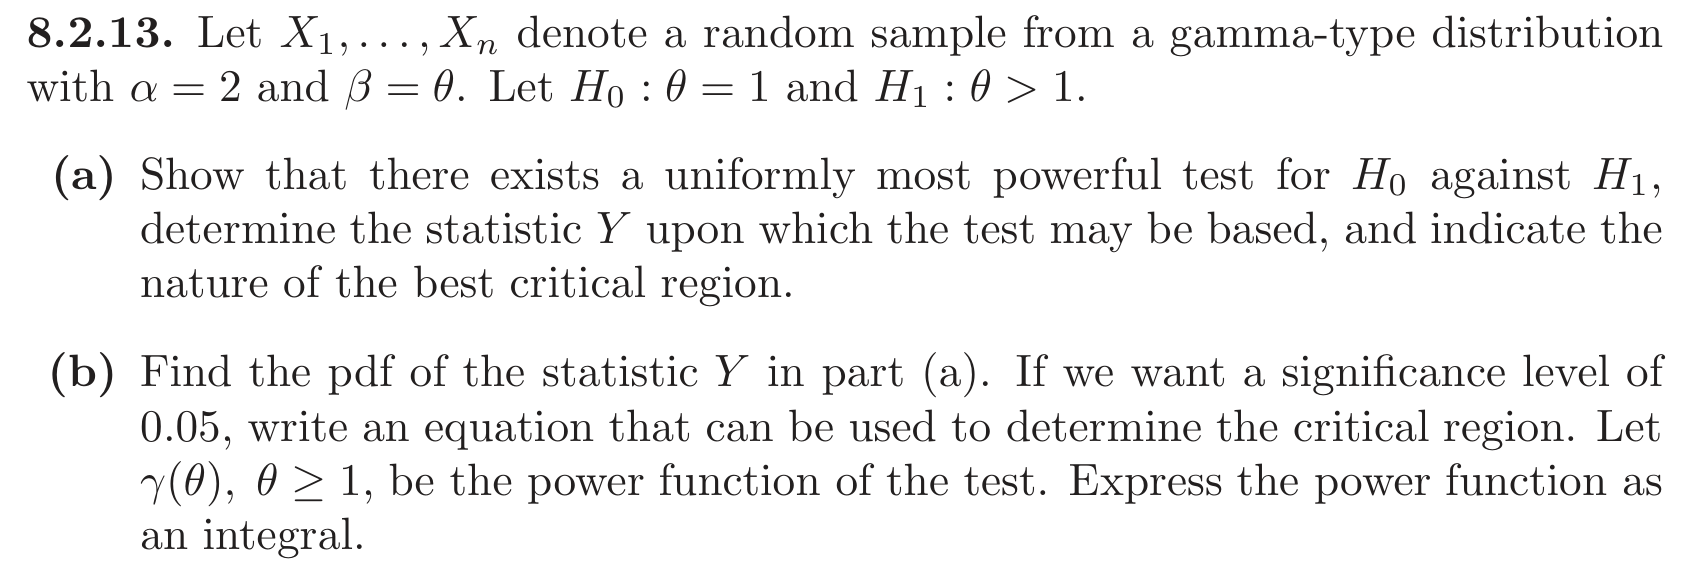
\includegraphics[width=\textwidth]{hw14-2025060521.png}
% \caption{}
\label{}
\end{figure}
\end{exercise}
(a)
$X_i\sim\Gamma(2,\theta)$, then
\[
f(x;\theta)=\frac{1}{\Gamma(2)\theta^{2}}xe^{ -x/\theta  }=\exp \left\{  -\frac{1}{\theta}x+\log x-2\log\theta  \right\}
\]
$-\frac{1}{\theta}$ is increasing, then $Y=\sum_{i=1}^{n}X_i$ is a UMPT for $H_0:\theta=1$ against $H_1:\theta>1$. The best critical region is $Y\geq c$.

(b)
$Y=\sum_{i=1}^{n}X_i\sim\Gamma(2n,\theta)$. The pdf of $Y$ is
\[
f_{Y}(y;\theta)=\frac{1}{\Gamma(2n)\theta^{2n}}y^{2n-1}e^{ -y/\theta  }
\]
Let the significant level be $0.05$, then
\[
0.05=\mathbb{P}_{H_0}(Y\geq c)
\]
Then
\[
c=F^{-1}_{\Gamma(2n,1)}(0.95)
\]
The power function is
\[
\gamma(\theta)=\mathbb{P}_{H_1}(Y\geq c)= \int_{c}^{+\infty} \frac{1}{\Gamma(2n)\theta^{2n}}y^{2n-1}e^{ -y/\theta  } \, \mathrm{d}y
\]